\section {Tuples}

Tuples are anonymous structures that store a set of data of different types.
They are described as a list of types enclosed in parentheses (e.g.
\token{(i32, f32, c8)}). A tuple may have only one inner type, in which case
the token \token{,} is added after the definition of the inner type (e.g.
\token{(i32,)}).

\subsection {Literals}

Tuple literals are described as a list of values enclosed in parentheses, for
example \token{(1, 'r', false)} is a tuple literal whose type is \token{(i32,
  c32, bool)}. Tuples containing only one value must have the token \token{,}
after the declaration of the value to distinguish them from priority operations
enclosed in parentheses.

\begin{lstlisting}[style=coloredverbatim]
let a = (1, 'r', false);
let b : (i32,) = (23,); // tuple value
let c : i32 = (23); // int value
\end{lstlisting}

\noindent Tuple inner values are constructed in the order in which they are
written. In the following example, the function \token{foo} is called before
the function \token{bar}.

\begin{lstlisting}[style=coloredverbatim]
fn foo ()-> i32 {
  println ("In foo.");
  12
}

fn bar ()-> f32 {
  println ("In bar.");
  34.0f
}

let a = (foo (), bar ());
\end{lstlisting}

\subsection {Mutability and memory alignment}%
\label{sec:tuple_mutability}

The mutability of tuple values cannot be described as a level of mutability, as
might be the case for other compound types. In the case of tuples, mutability is
defined as a tree, where each node of the tree depends on the mutability of its
parent. For example, the mutability of the following tuple type \token{mut (mut
  i32, f32, dmut *c8)} is shown in the figure~\ref{fig:(chap4):tuple_mutability}.

\begin{figure}[H]
  \centering
  \scalebox{1.3}{
    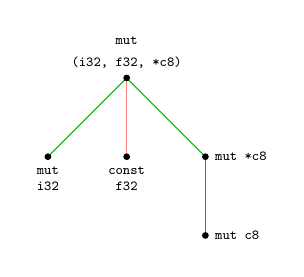
\begin{tikzpicture}

      \draw[-, black!30!green] (0,0) -- (-1,-1);
      \draw[-, red!50] (0,0) -- (0,-1);
      \draw[-, black!30!green] (0,0) -- (1,-1);
      \draw[-, black!30!green] (1,-1) -- (1,-2);

      \filldraw (0, 0.3) node[align=center, above] {\texttt{\tiny{mut}}};
      \filldraw (0, 0) circle (1pt) node[align=center, above] {\texttt{\tiny{(i32, f32, *c8)}}};
      \filldraw (-1,-1) circle (1pt) node[align=center, below]{\texttt{\tiny{mut}}};
      \filldraw (-1,-1.2) node[align=center, below]{\texttt{\tiny{i32}}};
      \filldraw (0,-1) circle (1pt) node[align=center, below]{\texttt{\tiny{const}}};
      \filldraw (0,-1.2) node[align=center, below]{\texttt{\tiny{f32}}};
      \filldraw (1,-1) circle (1pt) node[align=center, right]{\texttt{\tiny{mut *c8}}};
      \filldraw (1,-2) circle (1pt) node[align=center, right]{\texttt{\tiny{mut c8}}};


    \end{tikzpicture}
  }
  \caption{\label{fig:tuple_mutability} Example of tuple mutability}
\end{figure}


The mutability level of inner types is only important when they are borrowing
data. In the previous example shown in figure~\ref{fig:(chap4):tuple_mutability}, only
the mutability of the inner type \token{*c8} is important during data movement.
In other words, a value of type \token{mut (i32, f32, dmut *c8)} can be passed
to it without any problem. As with any borrowing type, the keyword
\token{alias} must be used when borrowing data.

\begin{lstlisting}[style=coloredverbatim]
let mut x = 't'c8;
let mut a : mut (mut i32, f32, dmut *c8) = (1, 12.0f, &x);
let mut b : mut (i32, f32, dmut *c8) = (1, 7.0f, null);

a = alias b; // no problem
b = alias a; // no problem either

let c : (i32, f32, *c8) = (1, 7.0f, &x);
a = alias c; // not allowed, it would dicard constant property of the third field
\end{lstlisting}

Tuple types with mutable values that don't borrow data are considered
non-borrowing types, and therefore don't need \token{alias} during data
movement. In practice, all the data of such a tuple is copied during data
movement.

The alignment of tuples follows the same rules as the alignment of structures
(see chapter~\ref{chap:structures}), basically they are just anonymous
structures.

\subsection {Properties}

Pointer type properties can be accessed by using the \token{::} operator on a
type expression. The properties are as follows:
\smallskip

\begin{center}
  \begin{adjustbox}{max width=\linewidth}
    \begin{tabular}{|l|ll|}
      \hline
      Name & Meaning & Type\\
      \hline
      \hline
      \texttt{init} & The inital value of the tuple & \texttt{usize} \\
      & where every inner field are set to \texttt{T::init} & \\
      \Xhline{0.001pt}
      \texttt{arity} & The number of inner elements of the tuple type & \texttt{usize}\\
      \hline
      \texttt{init} & A string encoding the name of the type & \texttt{[c8]} \\
      \hline
    \end{tabular}
  \end{adjustbox}
\end{center}

\smallskip

Inner types are not accessible using the \token{::} operator, but are
accessible using \token{\_\_pragma}. Pragmas are presented in the
section~\ref{sec:pragmas}.

\subsection {Binary operators}

Binary operators are divided into 3 groups:
\begin{itemize}
  \setlength\itemsep{-4pt}
\item Access: The operator \token{.} is used to access a given field of the
  tuple. The right operand must be of type int and must be within the range of
  \token{0} and the arity of the tuple to be accessed. The result of the
  operation takes the type of the field at the index described by the right
  operand, and so does the value. The first field index is \token{0}.

  \begin{lstlisting}[style=coloredverbatim, linewidth=0.95\linewidth]
let mut a : (mut i32, f32) = (8, 8.f);

a._0 = 7; // allowed first field is mutable
a._1 = 1.f; // not allowed, second field is not mutable

let c = a.(12 - 11); // accessing the field at index 1
  \end{lstlisting}

\item Comparison: The comparison operators \token{==} and \token{!=} are
  defined on tuples when each of the inner types are comparable. It compares all
  fields of two tuples and checks whether all inner values are equal for
  \token{==} or at least one inner value is different between the two operands
  for the operator \token{!=}.

  There is no relation of order between the tuples, even if they are of the same
  type, since in general such a comparison would be meaningless.

\item Affectation: The affectation operator creates a \textit{data movement}
  from the right operand to the left operand. Mutability must be respected when
  data is borrowed. Data mutability on tuples has already been introduced in
  section~\ref{sec:tuple_mutability}.

\end{itemize}

\subsection {Dollar operator}

The dollar operator can be used within an access binary operation in the right
operand expression. The dollar value takes the value of the arity of the tuple,
and its type is \token{usize}. Its value is known at compile time.

\begin{lstlisting}[style=coloredverbatim]
let a = (1, 9.0f, 'r');

let b = a.($ - 1us); // access the last value, i.e. 'r'
\end{lstlisting}

\subsection {Tuple expansion}

Tuples have a special operator called \token{expand} that turns them into a
list of parameters. Expanding a tuple is useful to create other tuples, or to
pass the data of the tuple as function parameters.

\begin{lstlisting}[style=coloredverbatim]
fn foo (a : i32, b : f32) {}

let a = (1, 5.f);

 // transform a into a list of values
let b : (i32, f32, c32) = (expand a, 't');

foo (expand a); // transform a into a list of parameters
\end{lstlisting}

Such an operation is done at compile time and is simply a rewrite that is less
verbose. In fact, in the previous example, the line \token{foo (expand a)} is
rewritten as \token{foo (a.0, a.1)}. The mutability level of the expanded
values is always \token{1}, which means that tuple expansion can never borrow
mutable data. Tuple expansions are useful in variadic template functions to
write generic operations on a list of variadic parameters. The above example produces the following Ymir Intermediate Language code.

\begin{lstlisting}[style=myilVerb]
frame : main::main ()-> void {
    let a : (i32, f32) = (1, 5f);
    let b : (i32, f32, c32) = (a.0, a.1, 't'c32);
    main::foo (a.0, a.1);
    b;
    <unit-value>
}
\end{lstlisting}

\subsection {Tuple deconstruction}

Tuple can be used to declare several variables at once, using the same
\token{let} declaration. We call this declaration a tuple deconstruction
because it splits the values of the tuple into a list of variables. Types of
variables inside tuple deconstruction can be specified the same way they would
be specified for normal variable declaration. This can be used to define more
complex levels of mutability.

\begin{lstlisting}[style=coloredverbatim]
  // a is mutable, but not b nor c
let (mut a, b, c) = (1, 't', 12.f);

assert (a == 1 && b == 't' && c == 12.f);

// With type specifications
let (mut d : i32, mut e : [mut f32 ; 2]) = (1, [1.f, 2.f]);
\end{lstlisting}

A variadic variable can be used as the last variable declaration in such a
deconstruction with the token \token{...}. In this case, it's type is always a
tuple that takes all the values in the tuple that are left and not associated
with other variables. The type of this last variable can be specified before the
token \token{...}.

\begin{lstlisting}[style=coloredverbatim]
let (a, b...) = (1, 2, 3);
assert (a == 1);
assert (b == (2, 3));

let (c, d...) = (1, 2);
assert (c == 1);
assert (d == (2,));

// With type specifications
let (e, f : (i32, f32)...) = (1, 2, 3.f);
\end{lstlisting}

The above example produces the following Ymir Intermediate Language code. Notice
that in YIL, the tokens \tokennolst{\#\{} and \tokennolst{\#\} } are used to declare a
set (a block of statements without lifetime). The variable lifetimes of \token{a}
and \token{b} are attached to the block declared by the function, not to the
set in which they are declared.

\begin{lstlisting}[style=myilVerb]
frame : main::main ()-> void {
    #{
        let a : i32 = 1;
        let b : (i32, i32) = (2, 3)
    #};
    core::exception::abort ((a == 1), (""s8)[]);
    core::exception::abort (((b.0 == 2) && (b.1 == 3)), (""s8)[]);
    {#
        let c : i32 = 1;
        let d : (i32,) = (2,)
    #};
    core::exception::abort ((c == 1), (""s8)[]);
    core::exception::abort ((d.0 == 2), (""s8)[]);
    #{
        let e : i32 = 1;
        let f : (i32, f32) = (2, 3f)
    #};
    <unit-value>
}
\end{lstlisting}

The mutability level of variables declared using tuple deconstruction can be
mutable by using the keywords \token{mut} or \token{dmut} on specific
variables of the tuple deconstruction (i.e. \token{let (dmut a, b) = alias
  t;}). In that case the right operand must match the mutability, and be aliased
explicitly.

\subsection {Tuple iteration}

Tuples are iterable types, allowing them to serve as the iterable value of a \token{for} loop.

\begin{lstlisting}[style=coloredverbatim]
let a = (1, 't', 89.0f);
for i in a {
    println (i);
}
\end{lstlisting}

In practice, because such an iteration would involve creating iterator variables
of different types, the iteration is unwound at compile time. The tuple value is
constructed only once before entering any loop body, resulting in the following
Ymir Intermediate Language code.

\begin{lstlisting}[style=myilVerb]
frame : main::main ()-> void {
    let a : (i32, c32, f32) = (1, 't'c32, 89f);
    cte for {
        {
            let i : i32 = 1;
            {
                std::io::println!{i32}::println (i);
                <unit-value>
            }
        };
        {
            let i : c32 = 't'c32;
            {
                std::io::println!{c32}::println (i);
                <unit-value>
            }
        };
        {
            let i : f32 = 89f;
            {
                std::io::println!{f32}::println (i);
                <unit-value>
            }
        }
    }
}
\end{lstlisting}

If two variables serve as iterators, the first indicates the iteration index,
and the second signifies the value within the tuple. However, in the case where
only one variable is specified, it exclusively contains the value of the tuple
field corresponding to the current iteration's index.

\begin{lstlisting}[style=coloredverbatim]
let dmut a = (1, 2, 3);
for i, _ in a {
    a.(i) = 9;
}

assert (a == (9, 9, 9));
\end{lstlisting}

More information about \token{for} loops is presented in Section~\ref{sec:for_loops}.

\subsection {Implicit casting}

Tuple literal values may contain literal values that can be implicitely
converted during compilation (e.g. integer literals, array literals, class
objects, etc.). In this case, the conversion is performed at \token{cte}
implicitely.

\begin{lstlisting}[style=coloredverbatim, escapechar=@]
// ok, '1' literal can be implicitely converted to '1us'
let mut a : (usize, usize) = (1, 2);

let mut i = 12;
a = @\hb{(i, i)}@; // error, 'i' is not cte, it cannot be converted to usize
\end{lstlisting}

This implicit casting is recursive and allowed for any inner values that might
be affected, but it only applies to tuple construction values, not to any tuple
values, even immutable ones.

\begin{lstlisting}[style=coloredverbatim, escapechar=@]
// No problem, '0' is converted implictely to '0us', and so on
let a : ([(usize, isize) ; 1], f32) = ([(0, 0)], 12.0);

// error, implicit cast is not allowed 'a' is not a tuple construction value
let b : ([(i32, i32) ; 1], f32) = @\hb{a}@;
\end{lstlisting}

\vfill%
\pagebreak
